\documentclass[11pt,letterpaper]{article}
\usepackage{fullpage}
\usepackage[top=2cm, bottom=4.5cm, left=2.5cm, right=2.5cm]{geometry}
\usepackage{amsmath,amsfonts,amssymb}
\usepackage{lastpage}
\usepackage[inline]{enumitem}
\usepackage{fancyhdr}
\usepackage{mathrsfs}
\usepackage{xcolor}
\usepackage{graphicx}
\usepackage{subcaption}
\usepackage{appendix}
\usepackage{hyperref}
\usepackage{titlesec}
\usepackage{fancyvrb}
\hypersetup{ colorlinks=true, linkcolor=blue, linkbordercolor={0 0 1}}

\renewcommand{\arraystretch}{1.5}
\titlespacing*{\section}{0pt}{0.65\baselineskip}{0.5\baselineskip}

\setlength{\parindent}{0.0in}
\setlength{\parskip}{0.05in}

\newcommand{\qrf}{\texttt{QRFactor} }

\pagestyle{fancyplain}
\lhead{}
\chead{GPU Solutions for PSCAD: IT17112}
\rhead{}
\cfoot{\small\thepage}
\headsep 32pt

%%%%%%%%%%%%%%%%%%%%%%%%%%%%%%%%%%%%%%%%%%%%%%%%%%%%%%%%%%%%%%%%%%%%%%%%%%%%%%%
%%%%%%%%%%%%%%%%%%%%%%%%%%%%%%%%%%%%%%%%%%%%%%%%%%%%%%%%%%%%%%%%%%%%%%%%%%%%%%%

\begin{document}
\begin{center}
    {\Large \bf Monthly Summary: September, 2020}
\end{center}

The primary goal of the work this month was the development of an interface between existing PSCAD code and \verb+QRFactor+. This process required a fundamental shift in the implementation of \verb+QRFactor+ from a more standard, single-file CUDA project to a more object-oriented approach. In figure~\ref{f:OO}, we present a schematic of the structure of the QRFactor class.

See Chapter 6 in the CUDA \href{https://docs.nvidia.com/cuda/pdf/CUDA_Compiler_Driver_NVCC.pdf}{NVCC Guide}. 

\href{https://developer.nvidia.com/blog/separate-compilation-linking-cuda-device-code/}{Example} of separate compilation and linking with mixed host and device functions.

\begin{figure}[ht]
    \centering
    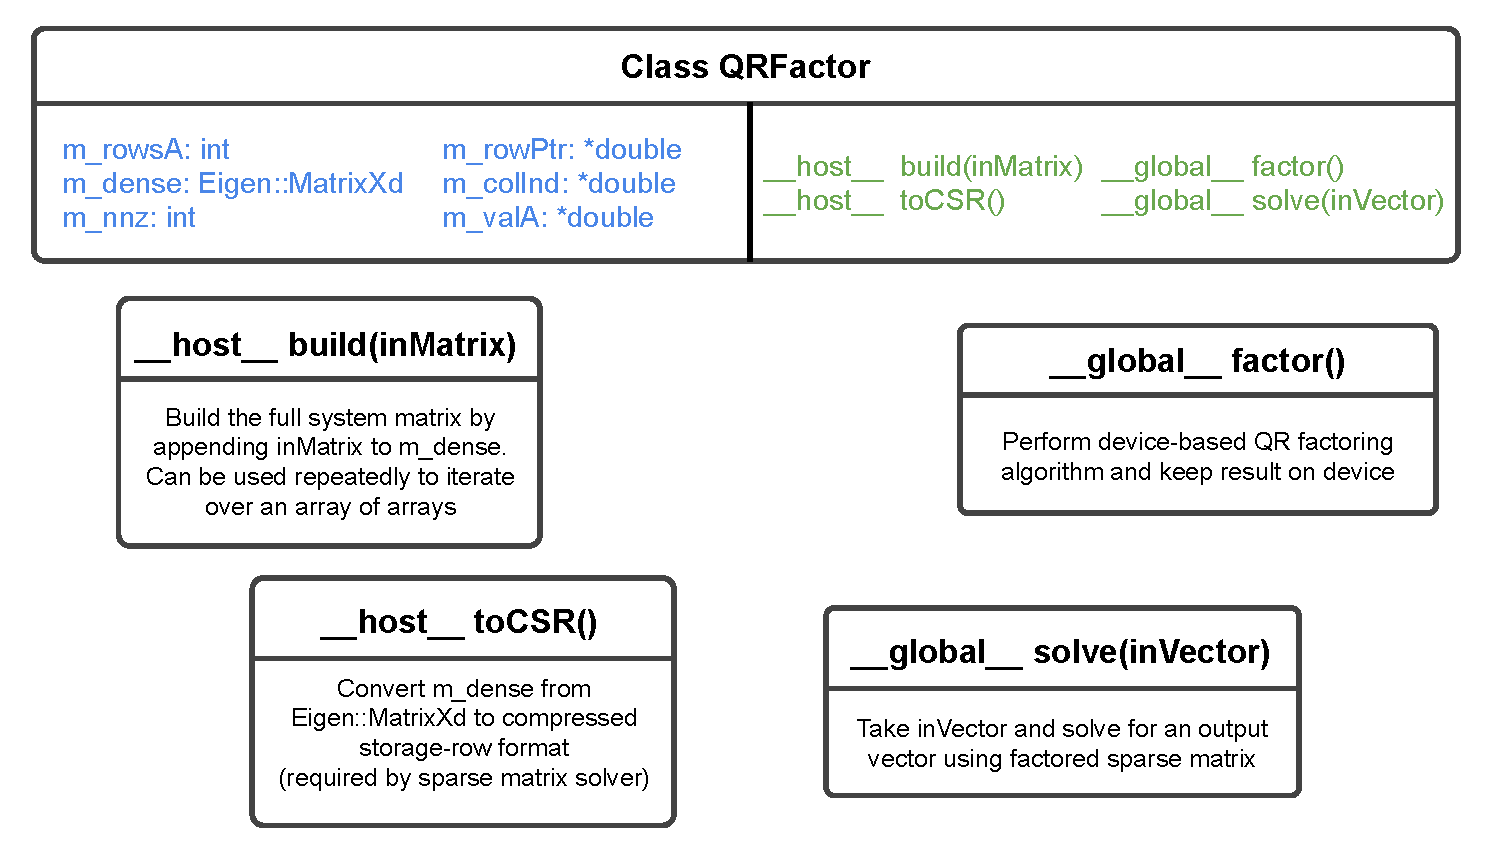
\includegraphics[width=0.75\textwidth]{MHI QRFactor.pdf}
    \caption{Schematic of the QRFactor class. Class variables are shown in blue while class functions are shown in green.}
    \label{f:OO}
\end{figure}



%%%%%%%%%%%%%%%%%%%%%%%%%%%%%%%%%%%%%%%%%%%%%%%%%%%%%%%%%%%%%%%%%%%%%%%%%%%%%%%
%%%%%%%%%%%%%%%%%%%%%%%%%%%%%%%%%%%%%%%%%%%%%%%%%%%%%%%%%%%%%%%%%%%%%%%%%%%%%%%































\end{document}
